%!TeX encoding=utf8
\section{Bose Einstein Condensate}

\subsection{Questions}
\begin{itemize}
         \item $\int \frac{1}{r^{n}} \mathrm{d^{3}r}$ divergent just for $n \leq 3 $ ?
        {\color{red}
            Yes. Apart from an angular part, the integral goes as $\int dr \frac{1}{r^{n-2}}$. If you integrate  till $R$ (which you will tend to infinity), then you can easily see that for $n=3$ it diverges as
            $\ln(R)$. For any other $n$ is goes as $R^{3-n}$, and hence it converges for $n>3$, and diverges for $n<3$.
        }
        {\color{green} Thanks.}
        
        \item What is an s-wave?
        {\color{red} $s$-wave means angular momentum $l=0$}.
        {\color{green} Thanks.}

        \item if $l < \frac{n-3}{2}$, and like $k^{n-2}$ otherwise (Landau and Lishitz, 1977). For a van der
        Waals-like potential $(n = 6)$, only $l = 0$ (s-wave) matters at low energies. Whats with $l=0$? Lifschitz is a typo?
        {\color{red}
            $l=0$ is special. For $l=0$ the centrifugal barrier $\frac{\hbar^2l(l+1)}{2mr^2}$ vanishes. Intuitively you can see that for short-range potentials, like $1/r^6$ you need to
            be close to $r=0$, such that the particles see each other. If the kinetic energy is too low, then the kinetic energy is not enough to overcome the centrifugal barrier. As a result, only $l=0$, i.e. the $s$-wave,
            contributes.
        }
        {\color{green} Thanks.}

        \item In the notes: eq. 1.8 to 1.9 the commutator $[\psi, \psi^{\dagger}]$ was used, but from 1.9 to 1.10 Bogoliubov aproximation was used, why not directly on 1.8 ?
        {\color{red} It could have been done directly in 1.8.}
        {\color{green} Thanks.}

        \item What is the derivation of 1.11? Its a FFT, but what are the exact steps?
            {\color{red}
                First $\hat\psi(\vec r)=\sum_{\vec p} \hat a_{\vec p}\frac{e^{i\vec p\cdot\vec r/\hbar}}{\sqrt{V}}$, where $V$ is just a quantization volume, just to have the proper units.
                We will also Fourier-Transform the potential $V(\vec r-\vec r')=\sum \tilde V(\vec q)e^{i\vec q\cdot (\vec r-\vec r')}$. Then, you see that
                $$
                \int d^3r \int d^3r' V(\vec r-\vec r') \hat\psi^\dag(\vec r) \hat\psi^\dag(\vec r')\hat\psi(\vec r')\hat\psi(\vec r)
                $$
                becomes of the form of Eq. (1.11), after using that $\frac{1}{V} \int d^3 r e^{i\vec k\cdot \vec r}=\delta(\vec k)$.
            }
            {\color{green}
                Thanks.
                \begin{equation*}
                  = \int d^3r \int d^3r' a_{p_{3}}^{\dagger} a_{p_{4}}^{\dagger} \delta\left(p_{2} - p_{4} - q\right) \delta\left(p_{1} - p_{3} + q\right) a_{p_{2}} a_{p_{1}} \\
                  = a_{p_{1} + q}^{\dagger} a_{p_{2} - q}^{\dagger} a_{p_{2}} a_{p_{1}} \\
                \end{equation*}
            }

        \item What are the python packages to use operators like $\hat{\psi}$? There is some sympy implementation, but probably there is a better one?
        {\color{red}
            I'm unsure what do you mean here. \\
        }
        {\color{green}
            We surely will use calculation with more complicated operators than diagonal matrices (complicated Hamilton operator). Which python packages you know for that? I know that sympy has implementations for operators for symbolic calculations.
        }
               
        \item how to get from 1.11 to 1.12? Is it a commutator expansion? Why $q$ is disappearing?
        {\color{red}
            This is based on the so-called Bogoliubov approximation. Since the system condenses in $\vec p=0$, you approximate $\hat a_0$ and $\hat a^\dag_0$ by $\sqrt{N_0}$,
            with $N_0$ the number of condensed atoms.  This is because $N_0\gg 1$. Actually $N_0\simeq N$, and hence the number of non-condensed atoms is much smaller than $N_0$.
            Then you will do the following. You will consider up to second order, i.e. up to terms with at most two operators $a_{\vec p}$ with $\vec p\neq 0$~(you will see that there
            are no terms with just one operator with $p\neq 0$).
            Let's have a look to the interaction term in Eq. (1.11) (I forget here hats and vectors in order to ease the notation) $a^\dag_{p_1+q}a^\dag_{p_2-q}a_{p_2}a_{p_1}$.
            Let's see which combinations you have that have at most 2 operators with a non zero momentum:
            $(p_1+q,p_2-q,p_2,p_1)=(0,0,0,0), (0,0,x,x), (x,x,0,0), (0,x,x,0), (x,0,0,x), (0,x,0,x), (x,0,x,0)$, where $x$ means that it is not zero. The first term gives you the energy at order zero: $E_0=\frac{U(0)}{2V}N_0^2$.
            Note that $N=N_0+\sum_{p\neq 0} a^\dag_pa_p$, and hence up to second order   $N^2=N_0^2+2N_0\sum_{p\neq 0} a^\dag_pa_p$. As a result:
            $E_0=\frac{U(0)}{2V}N^2 - U(0) n_0 \sum_{p\neq 0} a^\dag_pa_p$.
            The 3rd and 4th terms give $U(0) n_0 \sum_{p\neq 0} a^\dag_pa_p$ which cancels exactly with the term in $E_0$.
            The other terms will give you what you find in Eq. (1.12).
        }
        {\color{green}
            Alright, but why are there just $p$ and $-p$ in Eq. (1.12), but $p_{1}, p_{2}, q$ Eq. (1.11)?
        }

        \item In 1.17 $\omega_{\rho}$ part has a factor 2, but $\omega_{z}$ not, despite beeing symmetric in $\psi$. Why?
        {\color{red}
            This is because of the two directions on the plane.
        }
        {\color{green}
            Of course. Thanks.
        }

        \item What is variable $a$? Why should $a > 0$ as repulsive short-range interactions stabilize the BEC (p.10)?
        {\color{red}
            $a$ is the $s$-wave scattering length. It characterizes the short-range part of the interaction. As mentioned above the contact interaction is just described by what happens at $s$-wave.
            At low energies, this means that the short-range interactions are given by a single parameter, which is the scattering length. A positive scattering length means repulsive interactions, i.e. the interaction energy increases when the density increases, i.e. when the distances decreases (i.e. the particles repel each other). The opposite is true for $a<0$, for which the particle attract each other. The dipole-dipole interaction is partially atrtractive and partially repulsive. Attraction is dangerous, because the system tends to collapse. Adding repulsive contact interaction may compensate the dipolar attraction, hence preventing collapse.
        }
        {\color{green}
            Thanks. \textbf{May} compensate, means this is still under investigation?
        }

        \item ``When the atomic density grows due to the attractive interaction, three-body losses predominantly occur in the high-density region.'' What does three-body losses mean?
        {\color{red}
            Three-body losses means that three particles meet at close distances (which becomes more and more probable for larger and larger densities). When this occurs, two of the particles may
            fall into a bound state, giving the excess energy to the third one. As a result all three particle are loss from the system, and hence the term three-body loss.
        }
        {\color{green}
            Thanks.
        }

        \item ``As the collapse occurs mainly in the x-y direction due to anisotropy of the DDI (in the absence of inelastic losses, the condensate would indeed become an infinitely thin cigar-shaped cloud along z),
        and therefore the condensate explodes essentially radially, producing the anisotropic
        shape of the cloud.'' Why is the collaps not along z axis?
        {\color{red}
            Note that the dipoles attract each other when placed head with tail, i.e. in this case when they are placed aligned on top of each other along the $z$-direction. Hence collapse produces a thin "cigar" along $z$. However, before this "cigar" becomes infinitely thin, three-body losses kick out. When this occurs, the kinetic energy on the $xy$ plane, which is huge (due to the strong compression, recall Heisenberg uncertainty), is released and the BEC explodes. A note here: the key point of all the droplet business in recent works (starting in 2016) is that the collapse in a dipolar condensate may be actually stopped due to the stabilizing effect of quantum fluctuations, but this wasn't known when I wrote the notes!
        }
        {\color{green}
            Thanks.
        }
        
        \item How are the regions stable, metastable, unstable derived in Figure 1.5, here Figure \ref{fig:acrit}? 
        {\color{red}
            It comes from the two solutions of Eq. (1.25).
        }
        {\color{green}
            Thanks.
        }

\end{itemize}

\begin{itemize}
        \item Typo in ``we obtain a 1D equation similar to the a GP equation'', just the or a
        \item ``ground-state wave-function is independent of the in-plane coordinates '' Why?
        \item 1.26 to 1.27, where does the $U_{dd}$ go?
        \item Typo If: ``roton momentum. if this were so''
        \item Why should a modulation with a finite wavelength allow superfluids?
        \item Typo repeatance: ``the width of the width''
        \item What are the spin-F matrizes?
        \item Is the occurance of these spin textures in Figure \ref{fig:helical} special?
        \item ``In 3D system there exists a regime where no collective modes are below the chemical potential, which corresponds to the particle emission threshold $\Rightarrow$ excitation leads to self-evaporation of the droplet to zero temperature'' Is this a good/useful or is it just counter-productive for experiments? Meaning switching between this regime and a normal one to get probably higher densities?
        \item In Figure \ref{fig:collective} b, if the theoretical values would fit, then the dashed line would be where the darkest color is? If yes, why is it not?
        \item What are bright and dark solitons?
        \item What is meant by crossover between bright solitons and droplets?
        \item ``anisotropy of droplets leads to a frustration of the dipolar quantum droplet when
compressed along the magnetic field direction'' What does frustration mean in that context?
        \item ``multi-droplet states appear upon crossing into the bistable region, due to the fragmentation of the system following a modulational instability $\Rightarrow$ multi-droplet states are not the ground state'' Why is this following (what is the argument here)?
        \item What is in-situ density profiles?
        \item ``interference of multiple quantum droplets, allowing the characterization of the nearest- and next-nearest neighbour coherence'' Can this be seen in Figure \ref{fig:supersolids_exist}, if yes how?
        \item When running main.py with a rectangle pulse, centered around the potential, the result is NOT the ground state, instead an excited mode. Why

\end{itemize}


\begin{figure}[H]
    \centering
    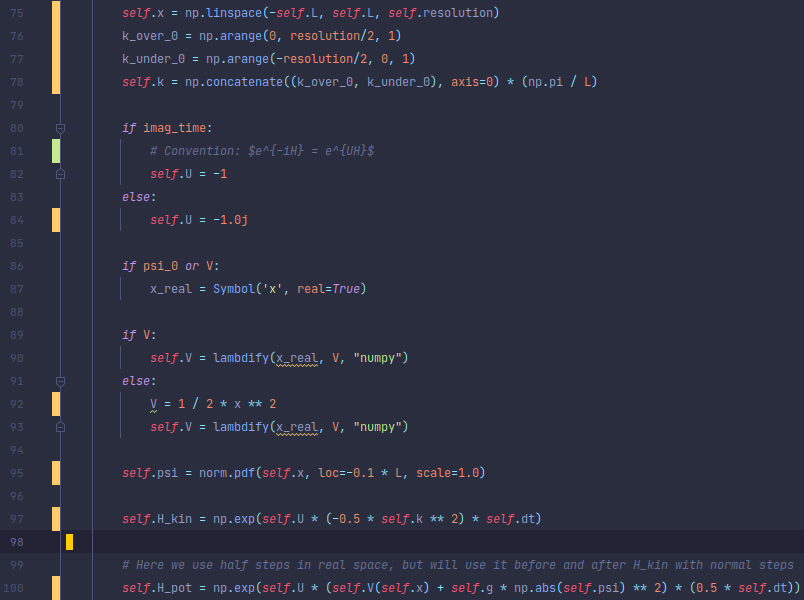
\includegraphics[width=1.0\textwidth]{IMAGE/find_the_error.png}\\
    \caption{
      The method from the first draft was implemented, but the resulting split\_time\_real.mp4 looks wrong (imaginary time works). Probably the error lies in the equations, that were used. Note that Strang-Splitting was used as in \ref{fig:strang_splitting}: Per timestep $H_{pot}$ was used before and after $H_{kin}$, but with just $0.5dt$.
      Also in that reference they used $\exp^{-iH}$, which seems right, instead of $\exp^{iH}$ in the draft.
      Note also the definition of self.k being a concatenation of [0:16] and [-16:0] as fft expecting (this fixed split\_time\_imag.mp4)
    }
    \textsc{Daniel Scheiermann},
    \emph{\url{split_operator.py}} (2020)
    \label{fig:find_the_error}
\end{figure}


\subsection{Summary}
\begin{itemize}
        \item dipol-dipol interaction (DDI):
        \begin{equation}
          U(r) = \underbrace{g \delta (r)}_{\frac{4 \pi \hbar^{2} a(d) \delta(r)}{m}} + \underbrace{U_{dd}(r)}_{\frac{C_{dd}}{4 \pi} \frac{(e_{1} \cdot e_{2}) r^{2} - 3(e_{1} \cdot r) (e_{2} \cdot r)}{r^{5}}}
        \end{equation}
        \item Use pseudo potential as dipol-dipol interaction is anisotropic and all partial wave (different l) mix
        \item coupling of different channels generates short-range contribution in the s-channel $s=0$ $\Rightarrow$ by changing DDI strength $a$ gets modified too $\Rightarrow$ shape resonances $\Rightarrow$ virtual state transform into a new ground state
        \item for fermions s-channel does not exists, so just long-range
        \item FFT of $U_{dd}$ using sperical harmonics $Y_{lm}$ gives:
        \begin{equation}
          \tilde{U_{dd}}(k) = \int \mathrm{d^{r} r} U_{dd}(r) e^{-ik \cdot r}= \frac{C_{dd}}{3}\left(3 \cos^{2}(\theta_{k}) - 1 \right)
        \end{equation}
        \item Use DDI in Gross-Pitajevski Equation, FFT, approximate to 2nd order, diagonalize with Bogoliubov transform
        \item As a result the square root can be imaginary, so the BEC gets dynamically unstable for long-wave length (phonon-instability):
            \begin{align}
              \epsilon(p) &= \sqrt{\frac{p^{2}}{2m} \left[\frac{p^{2}}{2m} + 2 n_{0} \left( g + \tilde{U_{dd}(p)} \right)\right]} \\
              &= p c_{s} \sqrt{1 + \epsilon_{dd} \left( 3 \cos^{2} \theta_{p} - 1 \right)} \\
              &\underset{p \rightarrow 0}{=} p c_{s} \sqrt{1 - \epsilon_{dd}}
            \end{align}
        \item For dipolar BEC the trap geometry is crucial (for non-dipolar not)
        \item ``pancake traps'' can stabilize the phonon-instability
        \item qualitative features for $a_{crit}(\lambda)$ by gaussian ansatz, for exact numerical solution non-local Gross-Pitaevskii Equation needed
\end{itemize}

\begin{figure}[H]
    \centering
    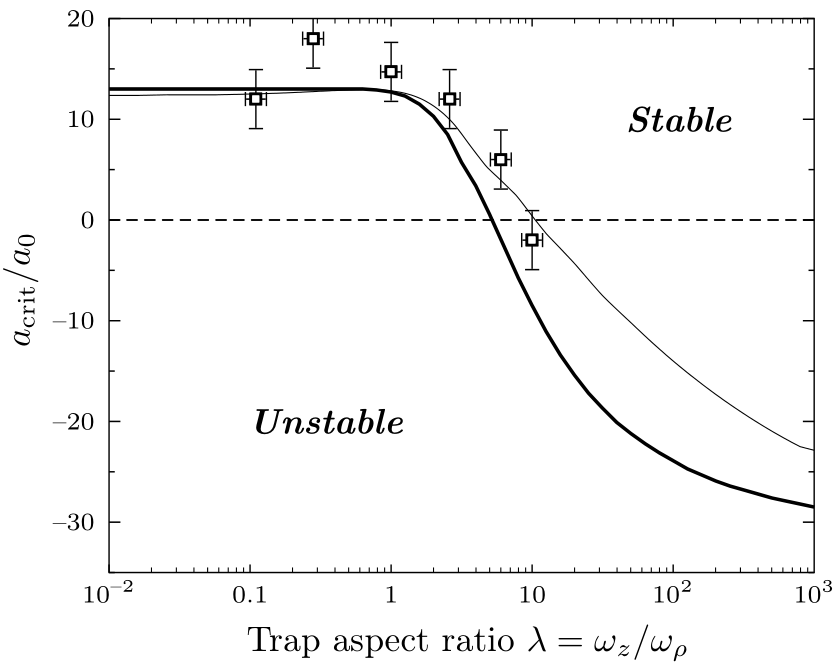
\includegraphics[width=1.0\textwidth]{IMAGE/acrit.png}\\
    \caption{Logo \autocite[1]{BOOK:1}}
    \textsc{Santos}, \emph{title} (year)
    \label{fig:acrit}
\end{figure}

\begin{figure}[H]
    \centering
    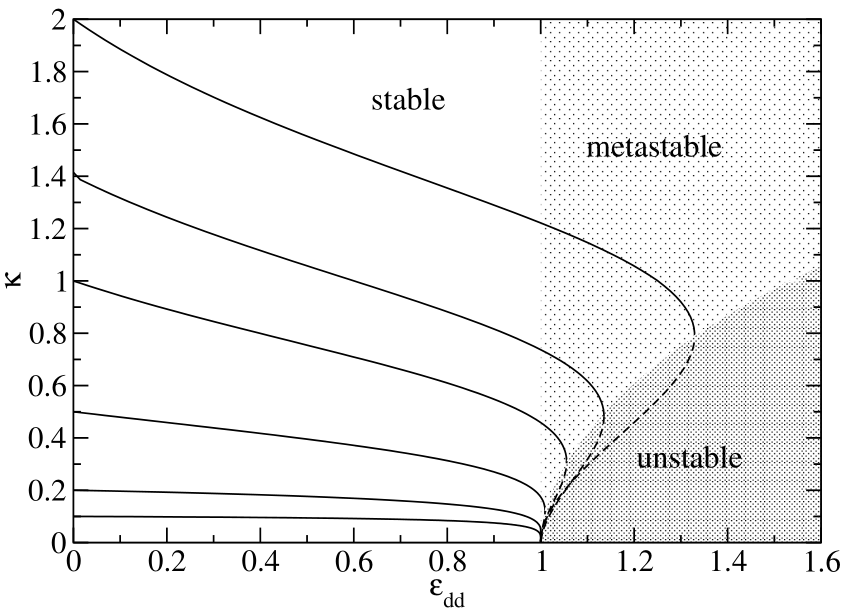
\includegraphics[width=1.0\textwidth]{IMAGE/stability.png}\\
    \caption{Logo}
    \textsc{Santos}, \emph{title} (year)
    \label{fig:stability}
\end{figure}

\begin{itemize}
        \item for sufficiently strong interactions, we may neglect quantum pressure, and consider the Thomas-Fermi (TF) regime
        \item TF solution for the trapped BEC has the same inverted parabola shape (as in non-dipolar case)
        \item BEC is prolat for $0 < \kappa < 1$ and $1 < \kappa$ oblat
        \item Bogoliubov-de Gennes Equation shows that the nonlocal character of the DDI causes a momentum dependend coupling constant, leading to a roton-like dispersion law, leading to dynamically instability, when the roton $\beta = \frac{g_{d}}{g}$ touches zero (experimetally not obeserved yet)
        \item by varying the density, the frequency of the confinement, and the short-range coupling,
        one can control the spectrum (roton minimum deeper/shallower)
        \item sequence of the non-local non-linearity 2D bright solitary waves may become stable
under appropriate conditions (Pedri and Santos, 2005)
        \item two instability regions for 2D solitons (against col-
        lapse and against unlimited expansion)
  \item $\tilde{g}_{cr}(\beta) \equiv \frac{g N_{cr}}{2 \pi l_{z}}$, so stable 2D anisotropic self-localised solitons exists just for $N < N_{cr}$
        \item non-dipolar BECs scatter elastically, the scattering of dipolar solitons is inelastic due to the lack integrability
        \item The solitons may transfer centre-of-mass energy into internal vibrational modes,
        resulting in intriguing scattering properties:

        \begin{itemize}
          \item including soliton fusion (Fig. 1.8)
          \item appearance of strong inelastic resonances
          \item possibility of observing 2D- soliton spiraling as that already observed in photo-refractive materials
        \end{itemize}

        \item Dipolar effects in spinor condensates
        \begin{itemize}
            \item spinor BECs: we focus on an effect which resembles the Einstein-de Haas effect
            \item Because of Zeeman sub-levels short-range interactions may occur in different s-wave scattering channels with different total angular momentum (for bosons even number) ( spin-1 bosons we have just F = 0 and F = 2)
            \item Each scattering channel has an associated s-wave scattering length $a_{F}$
            \item short-range interactions necessarily preserve the spin projection Sz
            \item DDI does not necessarily conserve the spin projection along the quantisation axis as DDI is anisotropic
            \item for initially maximally stretched state ($m_{F} =  - F$)
            \item short-range interactions cannot induce any spinor dynamics (due to conservation of total magnetisation $S_{z}$
            \item DDI may induce a transfer to $m_{F} + 1$
            \item for cylindrical symmetry around the quantisation axis, this violation of the spin projection is accompanied by a transfer of angular momentum to the centre of mass, resembling the well known Einstein-de Haas effect $\Rightarrow$ initially spin-polarised dipolar condensate can generate dynamically vorticity
            \item Einstein-de Haas effect is destroyed by weak magnetic fields (1 mG)
            \item the dominant Larmor precession, and invoking rotating-wave-approximation arguments, the physics must be constrained to manifolds of preserved magnetisation (2D optical lattices could help)
            \item Effect of DDI could be even observable under conserved $S_{z}$ (alkali spinor condensates)
            \item spin-changing collisions: collisions that conserve $S_{z}$, but do not conserve the relative population of the different Zeeman components
            \item Spin-changing collisions are characterised by an energy scale proportional
to the difference between scattering lengths at different channels
            \item this difference is very small, so can be significantly modified by the presence of other small energy scales (DDI) $\Rightarrow$ helical spin textures
        \end{itemize}
\end{itemize}

\begin{figure}[H]
    \centering
    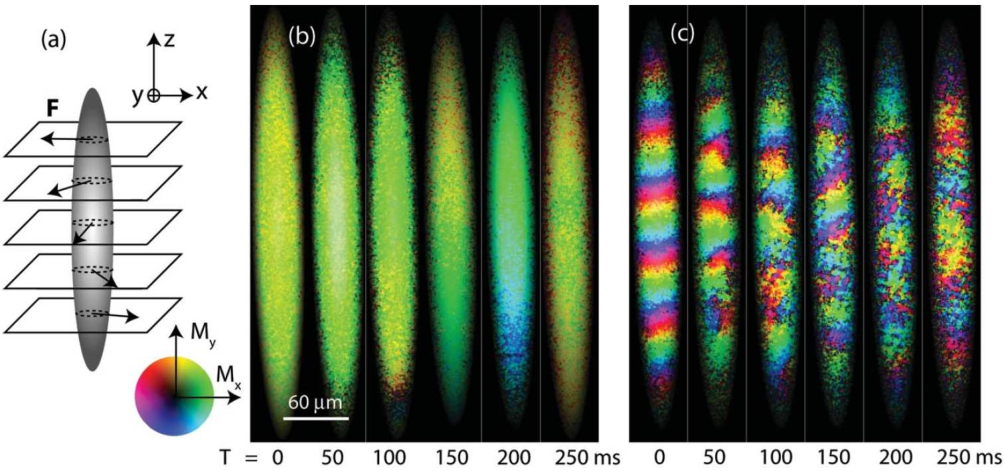
\includegraphics[width=1.0\textwidth]{IMAGE/helical.png}\\
    \caption{Is the occurance of these textures special?}
    \textsc{Santos}, \emph{title} (year)
    \label{fig:helical}
\end{figure}

\section{Supersolids}

\begin{itemize}
    \item supersolid: features both the crystalline structure of a solid and the frictionless flow of a superfluid
In this state, every constituent atom is part of the solid and the superfluid simultaneously
    \item direct observation was limited to systems where the structure formation was mediated by external light fields
    \item beyond mean-field approximation leads to corrections to the ground
state energy stemming from quantum fluctuations of the collective modes in a BEC (LHY-correction)
    \item In 2018 quantum droplets in a Bose-Bose mixture were observed

    \item Quantum droplets in Bose-Bose mixtures
    \begin{itemize}
        \item mean- field energy depends on the difference of the two coupling constants $\delta(g) = |g_{rep}| - |g_{att}|$ \item LHY-correction depends on the individual coupling constants
        \item For weakly attractive combination of interactions, a repulsive beyond mean-field correction can stabilize the BEC
        \item after a peak density increasing the number of particles only leads to an increase in the
    size of the droplet
        \item eGPE: kinetic energy, external trapping, and two-body interactions, LHY
        \item beyond mean-field correction has only been calculated for a homogeneous system and can therefore only be included within a local-density approximation
        \item QMC calculations in full many-body system verified the formation
        \item intra-species scattering lengths $a_{11}$ and $a_{22}$ lead to different equilibrium densities $n^{(i)}_{0}$ for the two components of the mixture.
        \item droplet forms an intrinsic imbalance in the atom numbers of the two components ($\frac{N1}{N2} = \sqrt{\frac{a_{22}}{a_{11}}}$ )
        \item larger density than in original BEC increases the rate of three-body loss $\Rightarrow$ extra term in eGPE
        \item[]
            \begin{equation}
              i \hbar \partial_{t} \psi = \left[ - \frac{\hbar^{2} \nabla^{2}}{2 m} + V_{ext}(r) + \alpha n_{0} |\psi|^{2} + \gamma n_{0}^{\frac{3}{2}} |\psi|^{3} \right] \psi
            \end{equation}
    \end{itemize}
\end{itemize}

\begin{figure}[H]
    \centering
    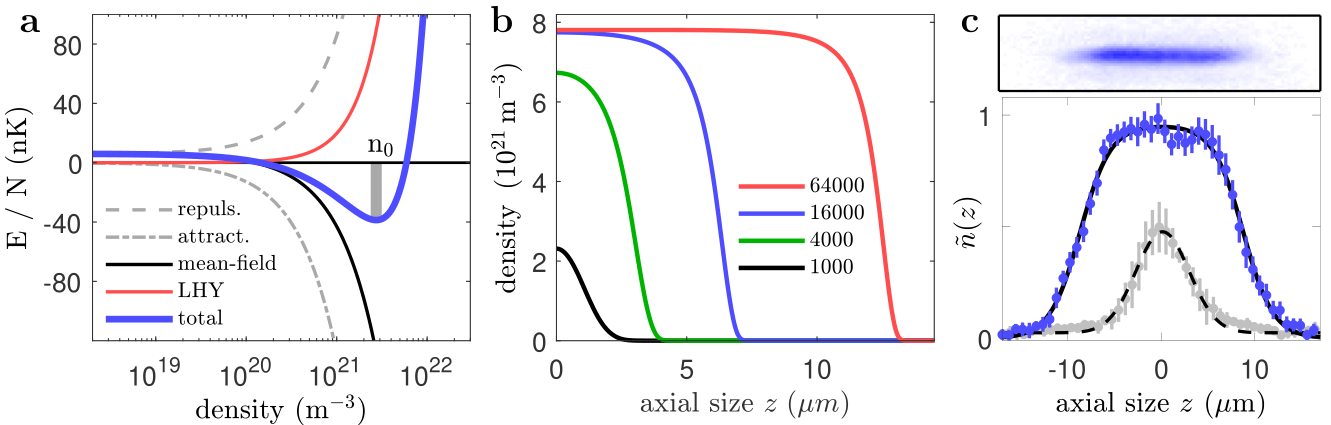
\includegraphics[width=1.0\textwidth]{IMAGE/droplet.png}\\
    \caption{Peak density of the droplet saturates in z-driection}
    \textsc{Santos}, \emph{title} (year)
    \label{fig:droplet}
\end{figure}

\begin{itemize}
    \item Dipolar Quantum droplets
    \begin{itemize}
        \item[]
            \begin{equation}
              i \hbar \partial_{t} \psi = \left[ - \frac{\hbar^{2} \nabla^{2}}{2 m} + V_{ext}(r) + g |\psi|^{2} + \phi_{dd} + g_{qf} |\psi|^{3} \right] \psi
            \end{equation}
    \end{itemize}
    \item Liquid-like density saturation appears indicating very low compressibility
    \item a droplet has $2.2 \cdot 10^{4}$ atoms
    \item the dynamical state after 5ms of evolution is a Gaussian density distribution
    \item most liquid-like aspect arises from the balance between attractive
        mean-field interaction and repulsive quantum fluctuations (self-bound nature)
    \item BECs and degenerate Fermi gases gaseous (expand release from trap)
    \item quantum droplets are self-bound ($N > N_{crit})$ caused by interplay between the binding mechanism and the kinetic energy cost of an inhomogeneous density distribution
    \item kinetic energy leads to an increase $E/N$, which for small atom numbers can be strong enough to drive a liquid-to-gas transition
    \item $N_{crit}$ experimental sequence:
        \begin{enumerate}
            \item prepare a quantum droplet with a high atom number
            \item external trapping potential switched off and the unavoidable process of three-body decay leads to a rapid loss of atoms.
            \item crossing the phase boundary to the gaseous state, the droplet turns into a gas and
                rapidly expands
            \item[$\Rightarrow$] significant reduction in the density suppressing further losses
            \item[$\Rightarrow$] settled at critical atom number $N_{crit}$ of a self-bound droplet (actual value  depends on the precise strengths of the two interactions involved)
            \item by varying the effective scattering length using Feshbach resonances, the phase diagrams can
                be mapped out
            \item residual confinement along the direction of gravity leads to a significant reduction of $N_{crit}$
        \end{enumerate}
\end{itemize}

\begin{figure}[H]
    \centering
    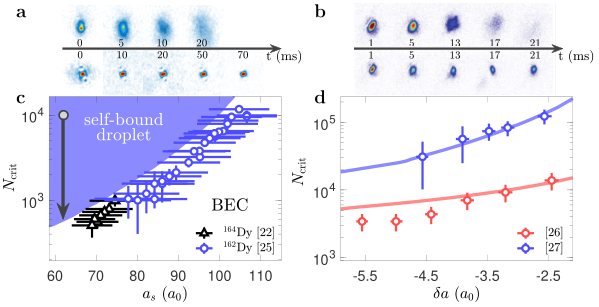
\includegraphics[width=1.0\textwidth]{IMAGE/self_bound.png}\\
    \caption{
            BEC and a self-bound quantum droplet in free space for a) the dipolar and (b) the Bose-Bose mixture. \\
            In the droplet regime, imaging aberations appear due to the high density and a spatial size of the droplets that is smaller than the experimental imaging resolution. Theoretical phase boundary between self-bound droplet and expanding BEC, together with the measured critical atom numbers for (c) the dipolar and (d) Bose-Bose droplets.
      }
    \textsc{Tilman Pfau et al.}, \emph{New states of matter with fine-tuned interactions: quantum droplets and dipolar supersolids} (2020)
    \label{fig:self_bound}
\end{figure}

\begin{itemize}
    \item For Bose-Bose mixtures excitations, where the components are in- or out-of- phase (to each other)
    \item collective modes would lead to exotic finite temperature behaviour of the binary droplets
    \item In 3D system there exists a regime where no collective modes are below the chemical potential, which corresponds to the particle emission threshold $\Rightarrow$ excitation leads to self-evaporation of the droplet to zero temperature (just for Bose-Bose)
    \begin{itemize}
        \item out-of-phase modes are expected to be overdamped (too energetic to be bound)
        \item No collective modes have been observed in Bose-Bose droplets (development of novel temperature probes needed)
        \item quantum droplets are self-bound objects (time-of-flight expansion temperature measurements for cold atoms cannot be applied)
    \end{itemize}
    \item In 1D quantum droplets the breathing mode always stays trapped (theoretically shown)
    \item dipolar case at least one collective mode is always expected to remain below the particle emission threshold
    \item In dipolar systems, measurements of collective excitations were obeserved
    \item an oscillation in the axial length of the droplet. Increase in the excitation energy upon approaching the transition (fits numerical simulations that include quantum fluctuations as the stabilization
mechanism for the droplets)
    \item Scissors mode: breaking of the rotational symmetry causes an angular oscillation of the droplet
around the polarizing magnetic field direction
    \item Scissor mode is an important marker of superfluidity (but moment of inertia of droplets does not differ significantly from the classical rigid due to the large anisotropy in their density distribution)
    \item scattering length comes from partial wave analysis, where one expands in the angular momentum components of the outgoing wave (similar to multipole expansion in Electrodynamic), it is related to the physically observable cross-section
\end{itemize}


\begin{figure}[H]
    \centering
    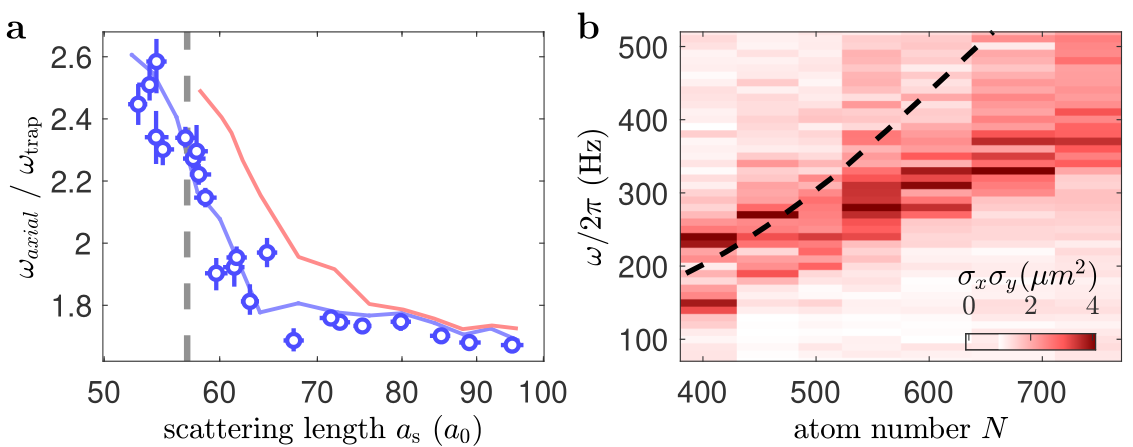
\includegraphics[width=1.0\textwidth]{IMAGE/collective_excitation.png}\\
    \caption{
      Measurements of the collective excitations of a dipolar quantum droplet.
      a) With stabilizing contribution of quantum fluctuations (blue) and without (red). \\
      b) Measurement of the scissors mode arising from the breaking of the
rotational symmetry in dipolar quantum droplets. Experimentally, the orientation of
the magnetic field is modulated at different frequencies and the response of the system
is observed by looking at the droplet sizes $\sigma_{x,y}$. Theoretical scissors mode frequency expected from linear response theory (dashed).
}
    \textsc{Tilman Pfau et al.}, \emph{New states of matter with fine-tuned interactions: quantum droplets and dipolar supersolids} (2020)
    \label{fig:collective}
\end{figure}


\begin{itemize}
    \item solitons emerge as a single particle effect (dispersion in the waveguide stabilizes the system against collapse
    \item quantum droplets are stabilized by many-body phenomenon (repulsive quantum fluctuations)
    \item solitons are only stable for effectively 1D gas (atom number $N < N_{crit\_soliton}$)
    \item quantum droplets can exist as a purely self-bound state in 3D (atom number $N > N_{crit\_droplet}$)
    \item Quantum droplets and solitons are distinct solutions of the eGPE
\end{itemize}

\begin{figure}[H]
    \centering
    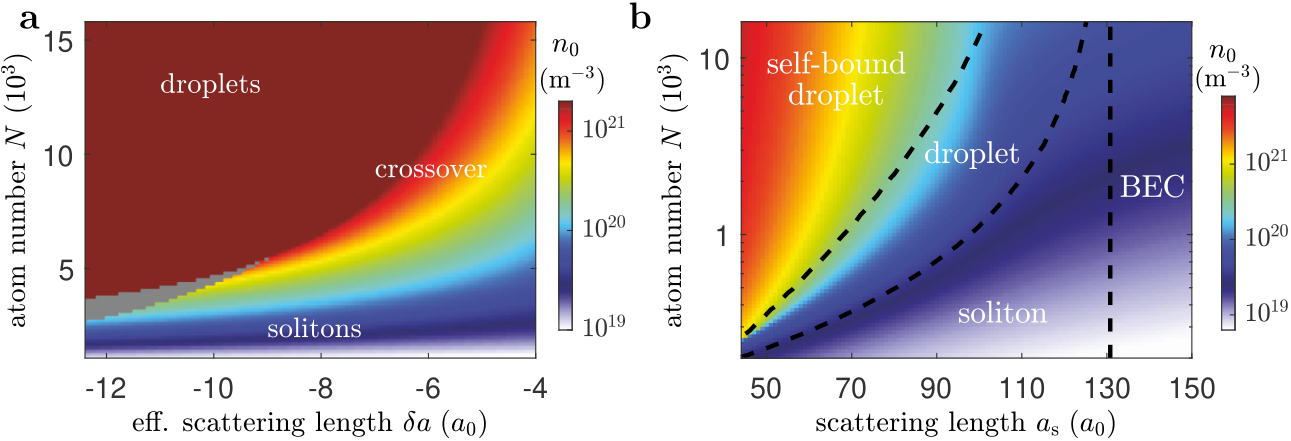
\includegraphics[width=1.0\textwidth]{IMAGE/droplet_soliton.png}\\
    \caption{
            Simulated phase diagram of the ground-state peak density as a function
            of the atom number and the (effective) scattering length for \\
            a) Bose-Bose mixture in a cigar-shaped confinement \\
            b) dipolar quantum gas in a pancake-shaped confinement. \\
            Solitons and droplets can coexist in a bistable region (gray) or can be smoothly connected by a crossover (dashed guide-line).
          }
    \textsc{Tilman Pfau et al.}, \emph{New states of matter with fine-tuned interactions: quantum droplets and dipolar supersolids} (2020)
    \label{fig:doplet_collision}
\end{figure}


\begin{itemize}
    \item anisotropy of droplets leads to a frustration of the dipolar quantum droplet when
compressed along the magnetic field direction and the emergence of arrays of dipolar
quantum droplets
    \item multi-droplet states appear upon crossing into the bistable region, due to the fragmentation of the system following a modulational instability $\Rightarrow$ multi-droplet states are not the ground state
    \item by confining a multi-droplet in a cigar-shaped trap it can be made the ground-state (confirmed experimentally)
    \item For large enough atom numbers, two-dimensional arrays of multiple quantum droplets eventually emerge as the ground state in cylindrically symmetric traps
\end{itemize}


\begin{figure}[H]
    \centering
    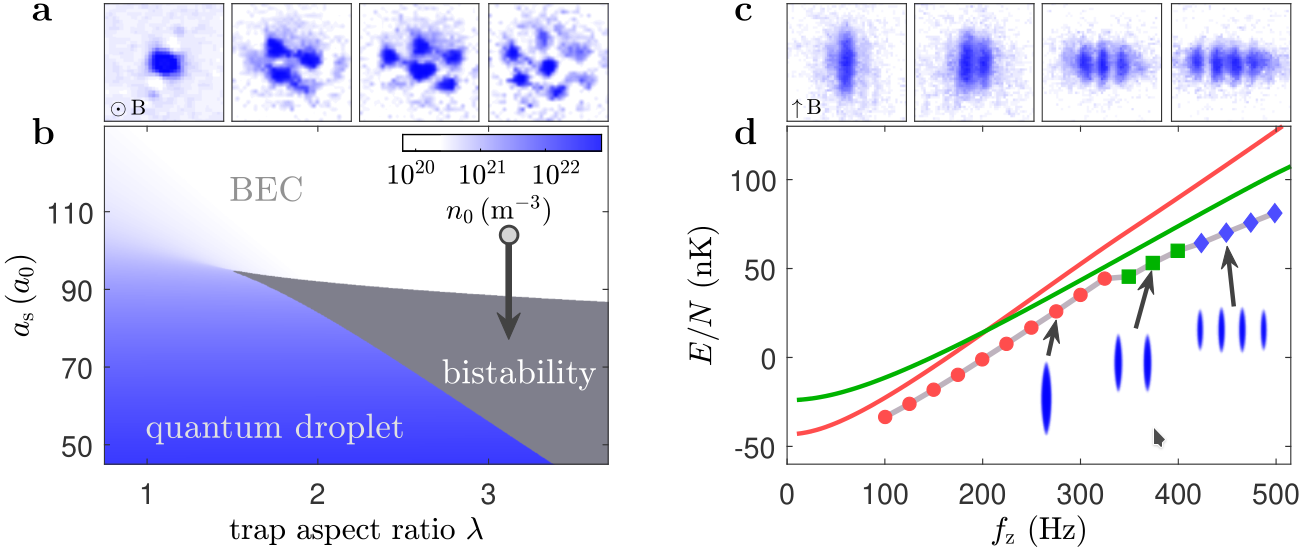
\includegraphics[width=1.0\textwidth]{IMAGE/external_trap.png}\\
    \caption{
        a) Example images of two-dimensional droplet arrays with increasing
atom numbers in a cylindrically symmetric trap [19, 112]. (b) Phase diagram of an
ensemble of 2.5 × 104 dysprosium atoms in a cylindrically symmetric trap with $\lambda = \frac{\omega_{z}}{\omega_{r}}$
        d) In cigar-shaped traps, it is energetically favourable for the droplet number to increase with increasing confinement along the polarization direction. \\
        c) Examples for this behaviour upon changing the in-plane trap geometry
        d) Total energy per particle $E/N$ for a single droplet (red), two droplets (green) and four droplets (blue) in an external trap with $\omega_{trap} = 2\pi (70, 1000, f_{z}$) Hz using a variational approach (lines) or numerical simulations of the eGPE (points).
      }
    \textsc{Tilman Pfau et al.}, \emph{New states of matter with fine-tuned interactions: quantum droplets and dipolar supersolids} (2020)
    \label{fig:external_trap}
\end{figure}

\begin{itemize}
    \item collisions after loading a two-dimensional array into a one-dimensional waveguide with only weak confinement along one direction (Figure \ref{fig:droplet_collision} a. The droplets initially repel
each other due to the repulsive dipole-dipole interaction. However, the weak confinement
along the waveguide axis forces the droplets to reverse their motion and collide with each
other. Figure \ref{fig:droplet_collision} b showing that the droplets bounce off each other twice. The oscillation of the droplets in the waveguide is strongly damped because of the relative motion between
droplets and the residual background atoms, and inelastic collisions.

    \item separated BECs are typically realized with a double-well potential
    \item for collision the barrier needs to be removed
    \item Controlling the time at which the radial and vertical confinement is turned off, the velocity can be precisely controlled
    \item critical velocity $v_{c}$ dividing the two outcomes of the collision (merging droplets and droplets bouncing off each other) depends on the mean atom number $\tilde{N}_{coll}$ of the two droplets
    \begin{itemize}
        \item $v_{c}\left(\tilde{N}_{coll}\right)$ dependence is very different for small and large droplets
        \item in a liquid-drop model the surface tension is the important energy scale for large droplets
        \item small droplets there is no distinction between bulk and surface and as such the relevant energy scale is the binding energy
        \item this can be seen as evidence of a crossover from a compressible quantum droplet at small atom numbers to a nearly incompressible droplet at large atom numbers
    \end{itemize}
\end{itemize}

\begin{figure}[H]
    \centering
    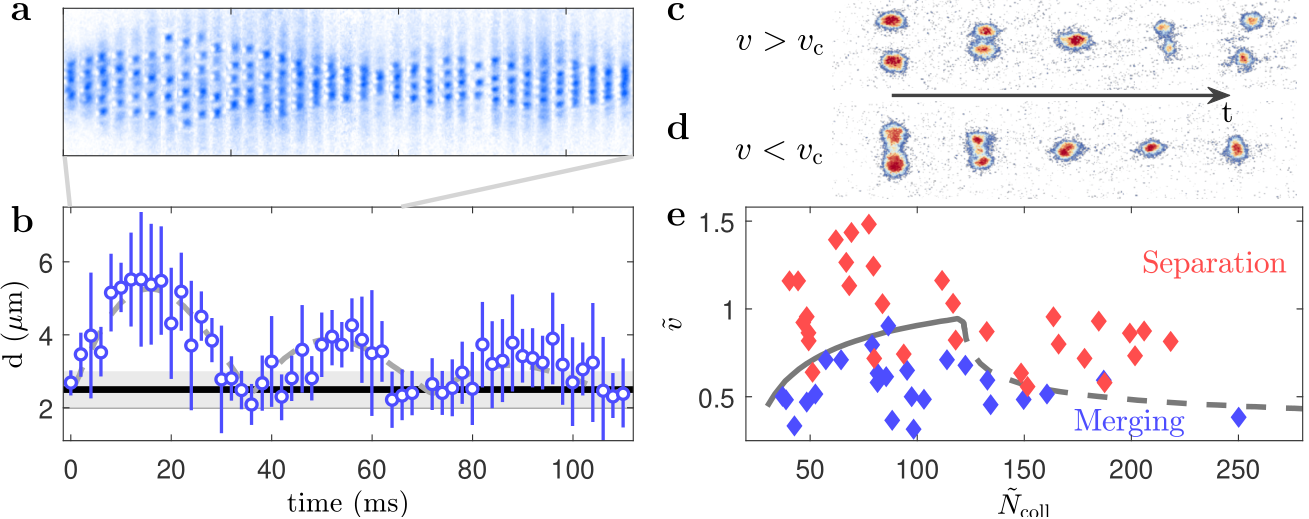
\includegraphics[width=1.0\textwidth]{IMAGE/droplet_collision.png}\\
    \caption{
            \textbf{Dipolar droplets:} \\
            a) Single-shot images of colliding dipolar quantum droplets for different evolution times. b) Mean droplet distance d as a function of the evolution time together with a guide to the eye representing a damped bouncing motion at the trap frequency (dashed gray line). \\
            \textbf{Bose-Bose droplets:} \\
            (c), (d) Example images of collision measurements of independently created binary quantum droplets resulting in (c) a separation and (d) a merger of the droplets. (e) Outcomes of different droplet collision measurements as a function of the relative velocity $\tilde{v}$ and the atom number $\tilde{N}_{coll}$ at the time of the collision, with the blue (red) diamonds indicating a merger (separation) of the droplets.
      }
    \textsc{Tilman Pfau et al.}, \emph{New states of matter with fine-tuned interactions: quantum droplets and dipolar supersolids} (2020)
    \label{fig:droplet_collision}
\end{figure}

\begin{itemize}
    \item self-organized droplet arrays break the continuous translational symmetry
    \item[$\Rightarrow$] supersolid state combines frictionless flow of a superfluid with the crystal-like periodic density modulation of a solid
    \item first experimental evidence for BECs coupled to external light fields, either exploiting cavity-mediated long-range interactions between the atoms or spin-orbit coupling
    \item there two continuous symmetries are broken, the periodicity of the density modulation is set by the external light field, and therefore allowing no propagating phonon modes.
    \item dipolar quantum gases can build droplet arrays in a self-organizing fashion and is based purely on the intrinsic interactions $\Rightarrow$ propagating phonon modes allowed
    \item to prove the coexistence of spatial order and superfluidity needs to be established
    \item initial experimets states rapidly lost their global phase coherence
    \item While each droplet itself is superfluid, the whole system is not
    \item theoretically an infinitely extended system showed the coexistence of superfluidity and spatial order for a narrow range of the scattering length close to the phase transition
    \item measurements showed indications of phase coherence in droplet arrays in a cigar-shaped trap geometry
    \item experimental results undoubtedly proved the coexistence of spatial order and global phase coherence
    \item in-situ density profiles in 3 regimes: isolated (incoherent arrays), phase-coherent droplet arrays, and a regular BEC
    \item transition characterized by the strength of the density modulation Figure \ref{fig:supersolids_exist} c
    \item interference of multiple quantum droplets, allowing the characterization of the nearest- and next-nearest neighbour coherence
\end{itemize}


\begin{figure}[H]
    \centering
    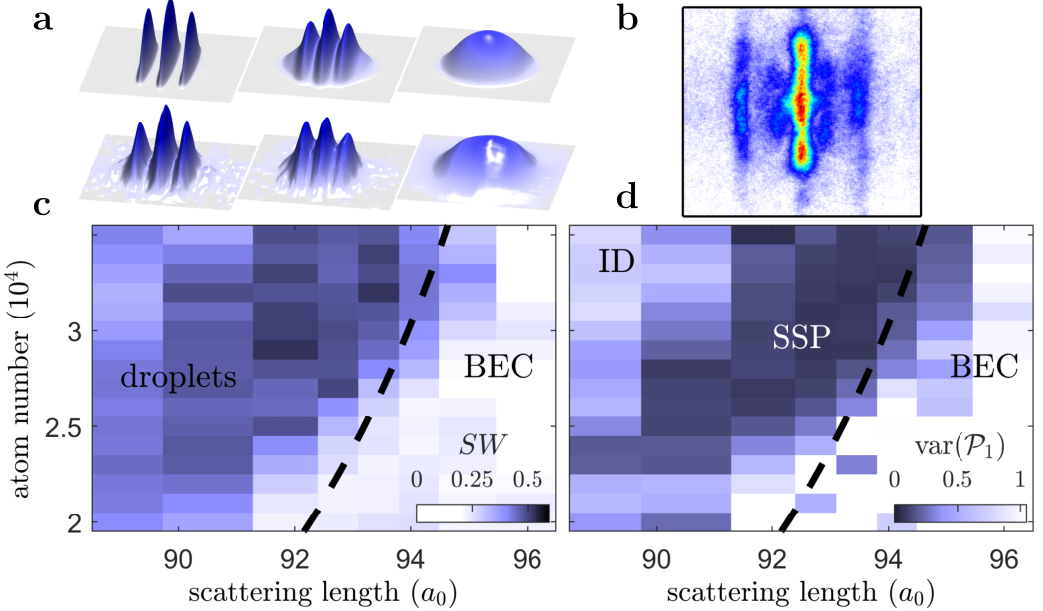
\includegraphics[width=1.0\textwidth]{IMAGE/supersolids_exist.png}\\
    \caption{
        a) Comparison of the theoretically (top) and experimentally (bottom)
        observed density profiles of an array of isolated droplets (left side), an array of quantum
        droplets immersed in a condensate background (center) and a regular BEC (right side)
        [67]. (b) Example image of the multi-wave interference in [34], showing the principal
        and minor interference fringes at a different spacing. (c), (d) Experimental signatures
        of the phase diagram for (c) the in-situ density modulation and (d) the nearest-
        neighbour coherence. The strength of the density modulation in (c) is characterized
        by the spectral weight SW, which compares the contribution of Fourier amplitudes at
        finite momentum to the zero momentum contribution. (d) The Fourier transforms of
        the interference patterns reveal clear side peaks at the length scale corresponding to
        nearest- and next-nearest neighbours. Phase coherence leads to a well-reproducible
        interference pattern and thus a vanishing variance of the amplitude of these side
        peaks.
        The variance of the nearest-neighbour peak var(P1) allows to differentiate
        between three regimes – isolated droplets (ID), phase-coherent droplets (supersolid
        phase, SSP) and a BEC. The black dashed line in (c) and (d) indicates the theoretical
        phase boundary obtained from numerical simulations of the eGPE. Adapted from
        [34, 67].
        of a time-of-flight interference measurement is shown in Figure 7b.
      }
    \textsc{Tilman Pfau et al.}, \emph{New states of matter with fine-tuned interactions: quantum droplets and dipolar supersolids} (2020)
    \label{fig:supersolids_exist}
\end{figure}

 
\begin{itemize}
    \item to prove supersolidity (superfluid nature) elementary excitations needed
    \item The breaking of a continuous symmetry at the superfluid-supersolid phase transition fundamentally
affects the spectrum of collective excitations
    \item[$\Rightarrow$] low-lying collective modes allow insights into the symmetry breaking and the supersolid nature
    \item energetically lowest mode is the dipole mode which is completely decoupled from interactions and always features an excitation energy corresponding to the trap frequency $\omega_{x}$
    \item Upon decreasing the scattering length, a softening of the roton
mode is observed
    \item roton mode is characterized by a minimum in the dispersion relation at a finite momentum and corresponds to a perturbative density modulation on top of the condensate density distribution
    \item In the considered trap geometry, the roton is comprised of two degenerate
modes – a symmetric and an anti-symmetric roton mode. As these roton modes soften,
avoided crossings are observed between pairs of modes with equal parity.
    \item softening of the roton triggers the phase transition to an array of quantum
droplets (occurs in this finite system as a finite excitation energy of the roton modes)
    \item degeneracy of the even and odd roton modes is lifted with the emergence of a density modulation in the ground state
    \item At smaller scattering lengths the excitation energy of the symmetric mode rapidly increases, whereas the excitation energy of the anti-symmetric mode further decreases.
    \item symmetric mode features an oscillation between the array and condensate background (understood as Higgs amplitude excitation of the supersolid array)
    \item Close to the phase transition, the amplitude mode exists in an isolated state because of the
energetic separation of the modes in the finite system
    \item The amplitude mode hybridizes with the other symmetric modes as its excitation energy increases.
    \item Close to the phase transition, collective modes with a larger excitation energy are affected by the rapidly increasing amplitude mode
    \item coupling of the higher symmetric modes with the amplitude mode leads to a bifurcation of the first quadrupole mode (after crossing the phase transition)
    \item higher-lying collective mode is scissors mode, decrease in the excitation energy upon crossing the phase transition (understood as a stiffening due to the emerging density modulation)
\end{itemize}

\begin{figure}[H]
    \centering
    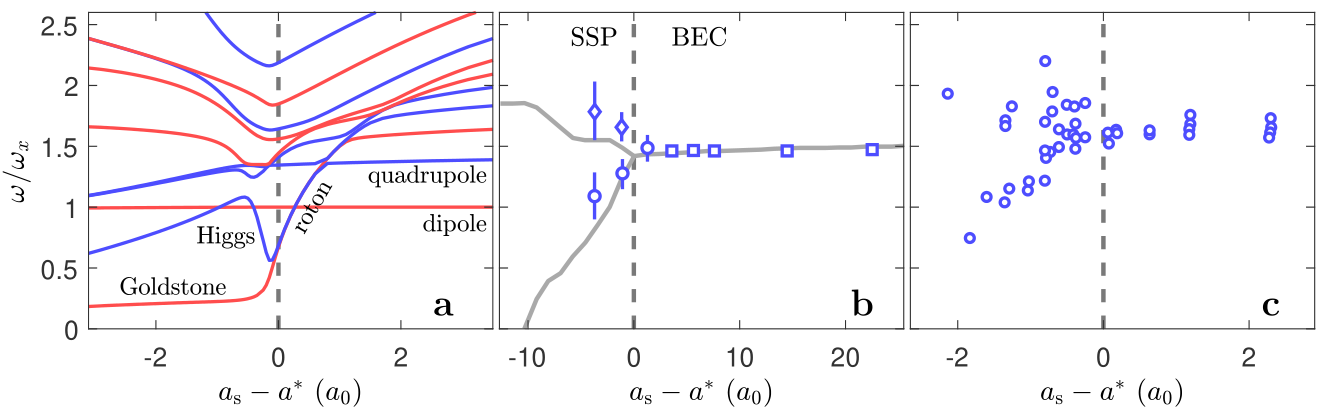
\includegraphics[width=1.0\textwidth]{IMAGE/collective_modes.png}\\
    \caption{
      a) Calculated excitation frequencies $\omega_{x}$ of the lowest collective modes across the phase transition from a BEC to an array of quantum droplets in
a cigar-shaped trap geometry with $\omega_{trap} = 2\pi [30, 90, 110]$ Hz.
The blue (red) lines
indicate an even (odd) parity of the density variation with respect to the weak
trapping direction x.
(b), (c) Signature of the phase transition in the excitation
energy of the axial quadrupole mode measured with (b)
162Dy and (c) 166Er.
The measurements were done using trap frequencies of $2 \pi [19(2), 53(2), 81(2)]$ Hz
and $2 \pi [259(2), 30(1), 170(1)]$ Hz for the case of dysprosium and erbium, respectively.
      }
    \textsc{Tilman Pfau et al.}, \emph{New states of matter with fine-tuned interactions: quantum droplets and dipolar supersolids} (2020)
    \label{fig:collective_modes}
\end{figure}

\begin{itemize}
    \item most closely related to superfluidity is the low-energy Goldstone mode that emerges out of the anti-symmetric roton mode
    \item it features an out-of-phase oscillation between array and superfluid background, involving Josephson-like dynamics between droplets
    \item Goldstone theorem: connects existance of Goldstone mode to double symmetry breaking at the phase transition
    \item interplay between crystal motion and superfluid counterflow preserves the center of mass and leads to a linear correlation between the array displacement $\delta x$ and the imbalance $\eta$ between the side droplets
    \item finite lifetime of array prevents time-resolved measurement of the mode (excitation leaves a trace
        on the spatial density distributions)
    \item This trace can be statistically mapped out by repeating the experiment many times, leading to the observed correlation between the imbalance and the displacement
\end{itemize}


\begin{figure}[H]
    \centering
    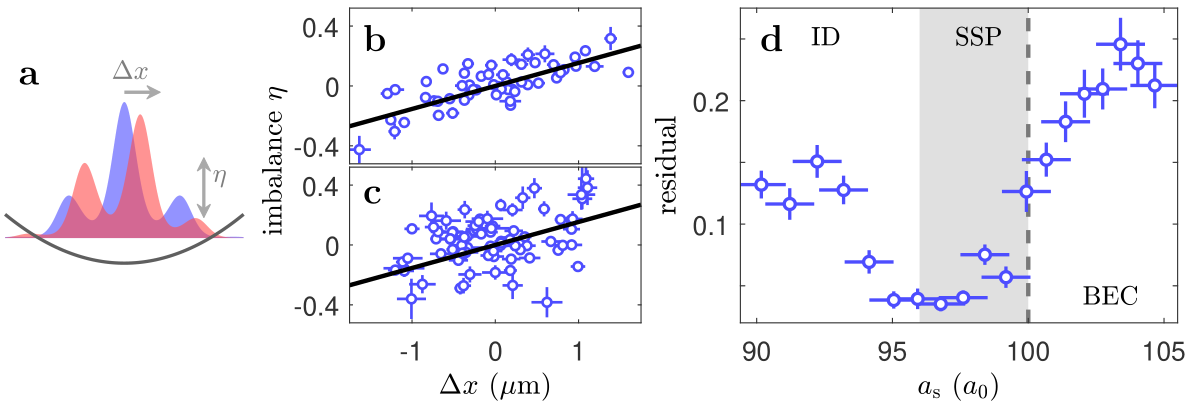
\includegraphics[width=1.0\textwidth]{IMAGE/goldstone_mode.png}\\
    \caption{
      a) Schematic of the low-energy Goldstone mode, featuring an out-of-phase
and center of mass preserving oscillation between the droplet array and the superfluid
background. A displacement of the droplet array by $\delta x$ leads to an imbalance $\eta$ in the
atom number of the side droplets. (b), (c) Measured imbalances $\eta$ as a function of the
measured displacements $\delta x$ in (b) the supersolid region and (c) isolated droplet region.
The black line shows the theoretically predicted correlation of the low-energy Goldstone
mode. (d) The low residual of the experimental data with respect to the theoretical
prediction close to the phase transition clearly proves the existence of the low-energy
Goldstone mode. The gray area indicates the phase-coherent region.
      }
    \textsc{Tilman Pfau et al.}, \emph{New states of matter with fine-tuned interactions: quantum droplets and dipolar supersolids} (2020)
    \label{fig:goldstone_mode}
\end{figure}

\section{Outlook}
\begin{itemize}
    \item $N_{crit}$, roton softening in dipolar gases show discrepancies between theory and experiments
    \item mean-field of eGPE is limited to the perturbative regime at small gas parameters
    \item quantum depletion and quantum correlations start to play a role at the
        large quantum droplet densities
    \item beyond mean-field correction originating from quantum fluctuations is typically included in the description through a local density approximation
    \item validity may not always be given for:
    \begin{itemize}
        \item long-range interaction
        \item close to a phase transition
        \item dense systems
        \item large dipolar strengths ($\epsilon_{dd} > 1$)
    \end{itemize}

    \item mean-field collapse leads to imaginary Bogoliubov modes, which are neglected (soft phonon mode for the Bose-Bose and roton mode for the dipolar system)
    \item Further improvement of theoretical description through:
    \begin{itemize}
        \item diagrammatic Beliaev technique
        \item behaviour in one-dimensional optical lattices
        \item hypernetted-chain Euler-Lagrange method
        \item Gaussian-state theory (includes squeezing effects)
        \item bosonic pairing
        \item inclusion of higher order corrections to the Bogoliubov speed of sound
        \item quantum Monte-Carlo (intrinsically include particle correlations, quantum fluctuations, a finite
system size, and a finite interaction range)
    \end{itemize}

    \item these methods are limited to the usage of a simplified interaction potential because they cannot handle the bound molecular states in the complete interaction potential
    \item low-dimensional systems to circumvent these fundamental problems
    \item in 1D the energy functional of Bose-Bose mixtures does not suffer from the aforementioned imaginary Bogoliubov mode (quantum Monte-Carlo studies found small deviations from the predictions of the eGPE)
    \item measurements of $N_{crit}$ and droplet density profile can be used as a sensitive benchmark for different theories in the near future
    \item in Bose-Bose self-evaporation to zero temperature has so far not been experimentally verified
  \item measurements of collective excitations are still lacking due to the finite lifetime in the experiments \item In dipolar droplets, the unavoidable presence of thermal fluctuations at finite temperatures has been proposed to increase $N_{crit}$ of a self-bound droplet (large scattering lengths, large atom numbers)
    \item validity of the Born approximation for the dipolar scattering problem has been called into question, which would result in a temperature dependent systematic shift of $N_{crit}$ to lower values
  \item Open questions:
    \begin{itemize}
        \item How general is the emergence of a supersolid state with respect to variations in the experimental parameters?
        \item How does finite temperature affect the supersolid phase transition?
        \item Upon evaporating into the supersolid state, are both symmetries broken simultaneously or sequentially?
        \item Do supersolid states exist in other systems, such as polar molecules ?
      \item eGPE as a mean-field theory should also not be the correct description for arrays of isolated droplets with no wave function overlap $\Rightarrow$ research needed for exact nature of supersolid-to-isolated-droplet-array transition
    \end{itemize}
\end{itemize}


\section{Simulations written in Python}

\subsection{First draft}
\begin{itemize}
    \item look into FFT artefacts
    \item GPE without Dipolar-Dipolar-Interactions
    \begin{equation}
        i \frac{\partial}{\partial t} \psi(x,t) = \left(\frac{-1}{2} \frac{\partial^{2}}{\partial x^{2}} + \frac{1}{2} x^{2} + \tilde{g} |\psi(x,t)|^{2} \right) \psi(x,t)
    \end{equation}
    \item dimensionless
    \begin{equation}
        \mu \phi_{0}(x) = \left(\frac{-1}{2} \frac{\partial^{2}}{\partial x^{2}} + \frac{1}{2} x^{2} + \tilde{g} |\phi_{0}(x)|^{2} \right) \phi_{0}(x)
    \end{equation}
    \item first use 1D later on 3D
\end{itemize}

\subsection{Further ideas}
\begin{itemize}
    \item for split-operator more precise Trotter-Suzuki decomposition of time evolution operator $U(t) = \exp^{\frac{-i H t}{\hbar} }$
    \item other method: Lanczos method (Krylov space)
    \item error $\propto E_{max}$ $\Rightarrow$ spectrum centering to lower errors
    \item accuracy is not uniform for all eigenstates $\Rightarrow$ Chebyshov method
    \item fft is implemented in scipy, sympy and numpy (research which one to use)
\end{itemize}


\begin{figure}[H]
    \centering
    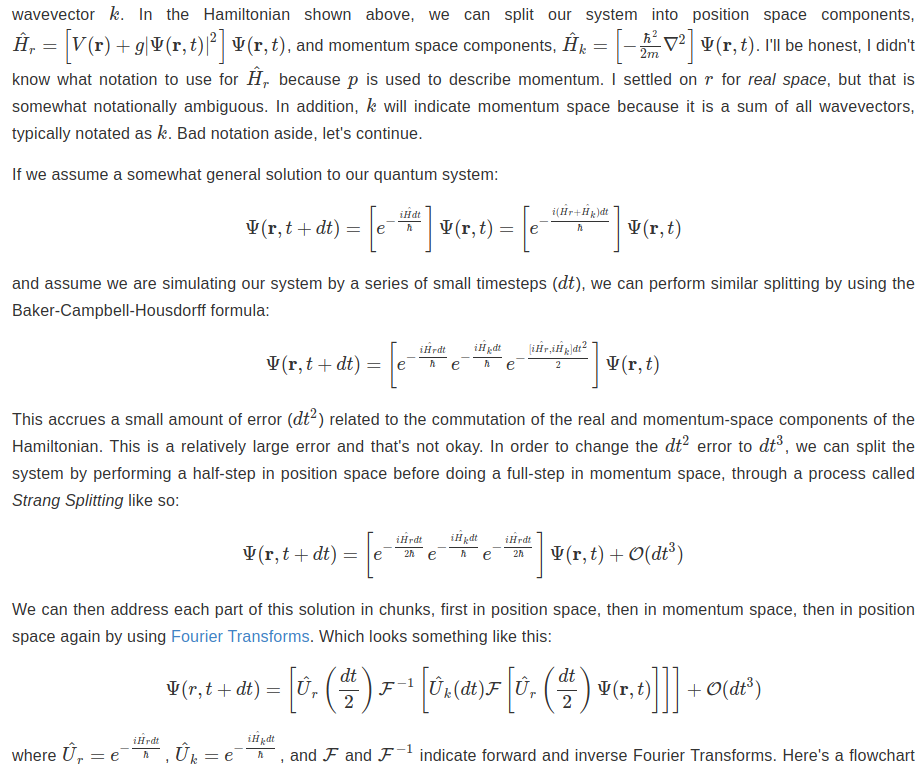
\includegraphics[width=1.0\textwidth]{IMAGE/strang_splitting.png}\\
    \caption{Logo}
    \textsc{James Schloss},
    \emph{            \url{https://www.algorithm-archive.org/contents/split-operator_method/split-operator_method.html}
    } (year)
    \label{fig:strang_splitting}
\end{figure}

\section{Goal}
Solve:
    \begin{equation}
        i \hbar \frac{\partial}{\partial t} \psi(r,t) = \left(\frac{-\hbar^{2}}{2 m} \nabla^{2} + V(r) + g |\psi(x,t)|^{2} \right) \psi(x,t)
    \end{equation}

\section{Experiments}
\begin{itemize}
    \item If the initial wave function $\psi_{0}$ is chosen badly, the ground state is not found
\end{itemize}
